\documentclass[12pt,a4paper]{article}

% ---------- Packages ----------
\usepackage[T1]{fontenc}
\usepackage[utf8]{inputenc}
\usepackage{mathpazo}
\usepackage[scaled=0.92]{helvet}
\usepackage{courier}
\usepackage[a4paper,margin=1in]{geometry}
\usepackage{amsmath,amssymb}
\usepackage{graphicx}
\usepackage{booktabs,tabularx,array}
\usepackage{enumitem}
\usepackage{xcolor}
\usepackage{tikz}
\usetikzlibrary{arrows.meta,positioning,calc}
\usepackage{caption}
\usepackage{titlesec}
\usepackage{fancyhdr}
\usepackage[hidelinks]{hyperref}
\usepackage{setspace}
\usepackage{float}
\usepackage{microtype}
\raggedbottom
\usepackage{needspace}
\clubpenalty=300
\widowpenalty=300
\predisplaypenalty=100

\definecolor{navy}{HTML}{1E3A8A}
\definecolor{accent}{HTML}{2563EB}
\definecolor{soft}{HTML}{DBEAFE}
\definecolor{grey}{HTML}{6B7280}

\titleformat{\section}{\Large\bfseries\sffamily\color{navy}}{\thesection}{0.8em}{}
\titleformat{\subsection}{\large\bfseries\sffamily\color{navy}}{\thesubsection}{0.8em}{}
\captionsetup{font=small,labelfont=bf}
\setlist{itemsep=2pt,topsep=4pt}
\renewcommand{\arraystretch}{1.25}
\onehalfspacing

\pagestyle{fancy}
\fancyhf{}
\fancyhead[L]{\small\sffamily Driver Drowsiness Detection}
\fancyhead[R]{\small\sffamily CS801 Mid-Semester Report}
\fancyfoot[C]{\small\thepage}
\renewcommand{\headrulewidth}{0.4pt}

\newcommand{\code}[1]{\texttt{#1}}

\begin{document}

% ---------- Title page ----------
\begin{titlepage}
\centering

\includegraphics[width=3.2cm]{nitk_logo.png}\par\vspace{0.6cm}
{\large\sffamily NATIONAL INSTITUTE OF TECHNOLOGY KARNATAKA, SURATHKAL\par}
{\sffamily Department of Computer Science and Engineering\par}
\vspace{1.6cm}
{\sffamily\color{grey} CS801 COMPUTING LAB \textbullet{} MID-SEMESTER PROJECT REPORT\par}
\vspace{0.8cm}
{\Huge\bfseries\sffamily\color{navy} Real-Time Driver Drowsiness Detection\par}
\vspace{0.3cm}
{\LARGE\sffamily\color{accent} with Condition-Aware Adaptive Signal Fusion\par}
\vspace{2cm}
{\large Submitted by\par}
\vspace{0.4cm}
\begin{tabular}{ll}
\toprule
\textbf{Name} & \textbf{Roll No.} \\
\midrule
Yagnang Acharya & 262IS037 \\
Akash Minz & 262IS002 \\
\bottomrule
\end{tabular}
\vspace{1.6cm}

{\large Course Instructor\par}
\vspace{0.3cm}
{\large Prof.\ P.\ Santhi Thilagam\par}
\vfill
{\sffamily October 2026\par}
\end{titlepage}

% ---------- Abstract ----------
\begin{abstract}
\noindent We have built a working real-time driver drowsiness detector that watches a single webcam and raises escalating alerts; this completes Phases~1 and~2 of our five-phase plan. The system tracks 478 face landmarks with MediaPipe and computes three cues on every frame: eye closure (Eye Aspect Ratio, EAR), yawning (Mouth Aspect Ratio, MAR) and head pose. A 5-second per-driver calibration sets the closed-eye threshold and the neutral head pose. Time-based indicators turn the cues into scores, which a fixed-weight fusion combines into one drowsiness score that drives a three-level alert system.

The project's contribution, due in Phase~3, is \emph{condition-aware adaptive fusion}: detecting low light and eye-region occlusion (such as glasses) and lowering the weight of cues that become unreliable under those conditions. The fixed-weight fusion built now is the baseline that adaptive fusion will be compared against. Detection accuracy has not been measured yet; Phase~4 evaluates both strategies on public datasets and self-recorded clips.
\end{abstract}

\newpage
\begin{singlespace}
\tableofcontents
\end{singlespace}
\newpage

% ---------- 1 ----------
\section{Introduction}

A drowsy driver reacts late or not at all, and a few seconds of eye closure at speed is enough to leave the lane. Detecting drowsiness early and warning the driver is therefore a direct safety measure.

Camera-based monitoring is attractive because it needs no contact with the driver: no wearable sensor, no electrodes, only a small camera facing the face. Three behaviours are visible from the face: the eyes closing for longer and more often, yawning, and the head nodding forward or tilting sideways.

Most camera-based systems combine these cues with fixed thresholds and fixed weights. That works in good conditions, but each cue fails in its own way in real driving. Eye landmarks become unreliable in low light or behind glasses, while yawning and head movement remain observable. A fixed weighting keeps trusting the eye cue exactly when it is weakest.

Our project addresses this with \textbf{condition-aware adaptive fusion}: estimate how reliable each cue is under the current conditions and weight it accordingly. This report describes the real-time system built so far, which provides every stage except the adaptive part, and the plan for the rest of the semester.

The project builds on our earlier undergraduate work (2023--24), a dlib-based detector that used the eye cue alone, with a fixed EAR threshold of 0.25 and a 20-frame counter. The current system replaces it completely.

% ---------- 2 ----------
\section{Literature Review}

The cues we use are well established; what is less studied is how to combine them when some of them become unreliable.

\begin{itemize}
\item \textbf{Eye Aspect Ratio.} Soukupov\'a and \v{C}ech~\cite{ear} proposed EAR, a ratio of six landmarks around each eye that drops sharply when the eye closes, for real-time blink detection. It is cheap to compute and is the most common eye-closure cue in landmark-based drowsiness work.
\item \textbf{PERCLOS.} The percentage of time the eyes are closed over a window is a widely used, validated measure of fatigue~\cite{perclos,ji}. Classic PERCLOS (P80) counts the eye as closed when the eyelid covers at least 80\% of the pupil.
\item \textbf{Yawning.} A wide mouth opening held for a sustained period is the usual vision cue for yawning; datasets such as YawDD~\cite{yawdd} were built for it.
\item \textbf{Head pose.} Nodding and drooping can be estimated from facial landmarks by fitting a 3D face model with a Perspective-n-Point solver (OpenCV \code{solvePnP}).
\item \textbf{Landmark tracking.} MediaPipe~\cite{mediapipe} provides a real-time face mesh of 468 points (478 with irises) that runs on a CPU, replacing older 68-point detectors such as dlib's.
\item \textbf{Multi-cue systems.} Ji, Zhu and Lan~\cite{ji} combined several visual cues to predict fatigue, showing that cues together are more robust than any one alone. Many later systems combine cues, but most fix the thresholds and weights once.
\end{itemize}

\paragraph{Gap addressed.} Fixed weights assume every cue is equally reliable all the time. Under low light or eye occlusion the eye cue degrades first, yet keeps its full weight. Our project targets this gap by making the weights depend on detected conditions.

% ---------- 3 ----------
\section{Problem Statement and Objectives}

\paragraph{Problem.} Build a real-time, camera-only drowsiness detector whose fusion of eye, mouth and head cues stays reliable when lighting drops or the eye region is occluded, and show by measurement whether adapting the fusion weights to conditions beats fixed weights.

\paragraph{Objectives.}
\begin{enumerate}
\item Extract EAR, MAR and head pose from a live webcam in real time (Phase~1, \textbf{done}).
\item Build a static-fusion baseline with calibration and a multi-level alert system, usable through a dashboard (Phase~2, \textbf{done}).
\item Detect low-light and eye-occlusion conditions and adapt the fusion weights to them (Phase~3, due at CE-2 on 1~November).
\item Compare adaptive fusion with static fusion on the same clips, reporting normal and adverse conditions separately (Phase~4).
\item Finish the dashboard, documentation and final report (Phase~5, end-semester).
\end{enumerate}

% ---------- 4 ----------
\section{Methodology}

Each video frame passes through six stages: landmarks, signals, calibration, indicators, fusion and alerts (Figure~\ref{fig:arch}). All timing is in seconds rather than frame counts, so behaviour does not depend on the camera's frame rate. Landmarks come from MediaPipe's FaceLandmarker (Tasks API), which returns 478 landmarks per face; up to two faces are detected and the largest is tracked as the driver.

\subsection{Per-Frame Signals}

\medskip\noindent\textbf{Eye Aspect Ratio.} For each eye, six landmarks $p_1,\dots,p_6$ (two corners, two upper-lid and two lower-lid points) give
\begin{equation}
\mathrm{EAR} = \frac{\lVert p_2 - p_6 \rVert + \lVert p_3 - p_5 \rVert}{2\,\lVert p_1 - p_4 \rVert}.
\end{equation}
The values of the two eyes are averaged. EAR falls towards 0 as the eye closes.

\medskip\noindent\textbf{Mouth Aspect Ratio.} The mean of three vertical inner-lip distances divided by the distance between the inner-lip corners:
\begin{equation}
\mathrm{MAR} = \frac{\tfrac{1}{3}\sum_{k=1}^{3} \lVert u_k - l_k \rVert}{\lVert m_L - m_R \rVert},
\end{equation}
where $(u_k, l_k)$ are upper/lower inner-lip pairs and $m_L, m_R$ the inner mouth corners. A wide-open mouth gives a high MAR.

\medskip\noindent\textbf{Head pose.} Six landmarks (nose tip, chin, outer eye corners, mouth corners) are matched to a generic 3D face model with OpenCV \code{solvePnP}, giving pitch (nodding), yaw and roll (sideways tilt) in degrees.

\subsection{Per-Driver Calibration}
For the first 5 seconds the driver looks ahead with eyes open. The median open-eye EAR and the median head angles become that driver's baseline. The closed-eye threshold is set to 75\% of the open-eye EAR, kept between 0.12 and 0.30, and head angles are measured relative to the neutral pose. This adapts the system to eye shape, glasses and camera position.

A baseline that does not look like open eyes facing ahead is rejected and calibration restarts: open-eye EAR below 0.20 or above 0.45, or head pitch beyond $25^\circ$. After 3 rejected attempts the default threshold (0.21) is used and a warning stays on screen.

\subsection{Time-Based Indicators}
Each cue becomes a score $S_i \in [0,1]$.

\begin{itemize}
\item \textbf{Eyes.} The higher of two scores: a PERCLOS-like closed-eye ratio over the last 20\,s (a ratio of 0.4 scores 1), and the length of the current closure (1.5\,s or more is a \emph{microsleep} and scores 1):
\begin{equation}
S_E = \min\!\left(1,\ \max\!\left(\frac{\text{closed ratio}}{0.4},\ \frac{\text{closure duration}}{1.5\,\mathrm{s}}\right)\right).
\end{equation}
A closure ends only after the eyes stay open for 0.15\,s, so one noisy frame cannot reset the timer. Because ``closed'' means EAR below 75\% of the open value, our ratio is looser than classic P80 PERCLOS and is not directly comparable with published PERCLOS values.
\item \textbf{Yawning.} A yawn is MAR above 0.5 held for at least 1.5\,s. The score is the number of yawns in the last 60\,s, with 3 yawns scoring 1.
\item \textbf{Head.} The time the head stays nodded forward by more than $15^\circ$ or tilted sideways by more than $20^\circ$, relative to the calibrated pose; 2\,s scores 1.
\end{itemize}

\subsection{Fusion}
The fused drowsiness score is a weighted average of the three indicator scores:
\begin{equation}
D_t = \sum_{i \in \{E, M, H\}} w_i \, S_i(t).
\end{equation}

\medskip\noindent\textbf{Static fusion (built).} Fixed weights: $w_E = 0.5$, $w_M = 0.2$, $w_H = 0.3$.

\medskip\noindent\textbf{Adaptive fusion (Phase 3).} The weights depend on the detected condition $C_t \in \{\text{Normal}, \text{Low-light}, \text{Eye-occluded}\}$. Each cue gets a reliability $R_i(C_t) \in [0,1]$, normalised into weights:
\begin{equation}
w_i(C_t) = \frac{R_i(C_t)}{\sum_j R_j(C_t)}.
\end{equation}
Both strategies share one interface in the code, so they can be run on identical inputs and compared directly. Under normal conditions adaptive fusion uses exactly the static weights, so any difference between the two comes only from adapting to conditions. Table~\ref{tab:weights} shows the initial example weights; final values will be set experimentally.

\begin{table}[htbp]
\centering
\caption{Initial example weights for adaptive fusion (to be tuned in Phase 4).}
\label{tab:weights}
\begin{tabular}{lccc}
\toprule
Condition & Eye & Mouth & Head \\
\midrule
Normal (= static) & 0.50 & 0.20 & 0.30 \\
Low light & 0.20 & 0.35 & 0.45 \\
Eye-region occlusion & 0.20 & 0.35 & 0.45 \\
\bottomrule
\end{tabular}
\end{table}

\subsection{Alerts}

\begin{table}[H]
\centering
\caption{Alert levels and their triggers.}
\label{tab:alerts}
\begin{tabularx}{\textwidth}{lXX}
\toprule
Level & Trigger & Action \\
\midrule
1 Warning & score $\ge 0.25$, or face not visible for 3\,s & On-screen warning \\
2 Alarm & score $\ge 0.45$, or a microsleep, or face not visible for 6\,s & Looping alarm sound \\
3 Critical & score $\ge 0.65$, or Level 2 held for 5\,s, or face not visible for 10\,s & Full-volume alarm, held for at least 5\,s \\
\bottomrule
\end{tabularx}
\end{table}

A hysteresis margin of 0.05 stops the level flickering near a threshold. Losing the face escalates to an alarm, because a slumped head or a blocked camera is exactly when the driver cannot be watched. Every level change is written to a timestamped CSV log.

% ---------- 5 ----------
\section{System Design and Implementation}

The system is an installable Python package, \code{drowsiness}, of about 2,200 lines across 14 modules.

\begin{figure}[H]
\centering
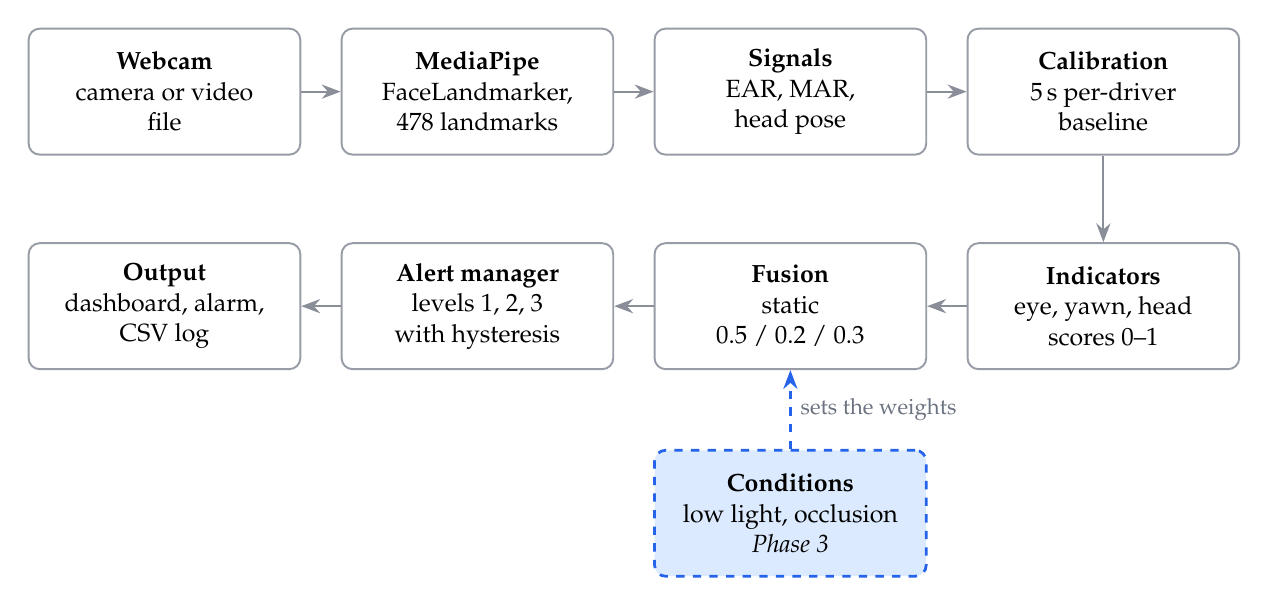
\begin{tikzpicture}[
  node distance=0.5cm and 0.5cm,
  stage/.style={draw=grey!70, rounded corners=4pt, line width=0.7pt, minimum width=3.45cm, minimum height=1.6cm, align=center, font=\small},
  plan/.style={stage, draw=accent, fill=soft, dashed, line width=1pt},
  arr/.style={-{Stealth[length=2.4mm]}, grey!80, line width=0.8pt}
]
\node[stage] (cam) {\textbf{Webcam}\\ camera or video\\ file};
\node[stage, right=of cam] (mp) {\textbf{MediaPipe}\\ FaceLandmarker,\\ 478 landmarks};
\node[stage, right=of mp] (sig) {\textbf{Signals}\\ EAR, MAR,\\ head pose};
\node[stage, right=of sig] (cal) {\textbf{Calibration}\\ 5\,s per-driver\\ baseline};
\node[stage, below=1.1cm of cal] (ind) {\textbf{Indicators}\\ eye, yawn, head\\ scores 0--1};
\node[stage, left=of ind] (fus) {\textbf{Fusion}\\ static\\ 0.5 / 0.2 / 0.3};
\node[stage, left=of fus] (alr) {\textbf{Alert manager}\\ levels 1, 2, 3\\ with hysteresis};
\node[stage, left=of alr] (out) {\textbf{Output}\\ dashboard, alarm,\\ CSV log};
\node[plan, below=1.0cm of fus] (cond) {\textbf{Conditions}\\ low light, occlusion\\ \emph{Phase 3}};
\draw[arr] (cam) -- (mp);
\draw[arr] (mp) -- (sig);
\draw[arr] (sig) -- (cal);
\draw[arr] (cal) -- (ind);
\draw[arr] (ind) -- (fus);
\draw[arr] (fus) -- (alr);
\draw[arr] (alr) -- (out);
\draw[arr, accent, dashed] (cond) -- node[right, font=\footnotesize, text=grey]{sets the weights} (fus);
\end{tikzpicture}
\caption{System architecture. Solid stages are implemented; the dashed condition module is Phase 3 and changes only the fusion weights.}
\label{fig:arch}
\end{figure}

\begin{table}[htbp]
\centering
\caption{Main modules of the \code{drowsiness} package.}
\label{tab:modules}
\begin{tabularx}{\textwidth}{>{\ttfamily}lX}
\toprule
\normalfont Module & Responsibility \\
\midrule
landmarks.py & MediaPipe FaceLandmarker wrapper, driver selection, model download \\
signals.py & EAR, MAR and head pose (\code{solvePnP}) \\
calibration.py & Per-driver baseline with rejection and retries \\
indicators.py & Closed-eye ratio and microsleep, yawns, head tilt \\
fusion.py & Fusion interface; \code{StaticFusion} baseline \\
alerts.py & Three-level alert state machine and CSV event log \\
pipeline.py & Per-frame orchestration into a frame report \\
video.py, audio.py & Camera or file input; alarm sound \\
overlay.py, recording.py & On-screen overlay; per-frame CSV recording \\
config.py & Typed TOML configuration with validation \\
cli.py, dashboard.py & Command-line interface and Streamlit dashboard \\
\bottomrule
\end{tabularx}
\end{table}

\needspace{6\baselineskip}
\paragraph{Interfaces.}
\begingroup\raggedright
\begin{itemize}
\item \code{drowsiness dashboard}: Streamlit page with live video, signal values, indicator scores, a score chart and the alert history. It listens only on the local machine by default, because the camera stream has no login.
\item \code{drowsiness run}: OpenCV window with overlay; \code{q} quits, \code{c} recalibrates.
\item \code{drowsiness process clip.mp4}: analyses a video file without a window and writes per-frame signals to CSV, for evaluation.
\end{itemize}
\endgroup

{\sloppy\paragraph{Configuration.} Every threshold, window and weight lives in one file, \code{configs/default.toml}. Values are range-checked when loaded.\par}

\paragraph{Privacy.} No images or video are stored. Only alert events and, on request, per-frame signal values are written to CSV.

\paragraph{Tools.} Python 3.11/3.12, MediaPipe, OpenCV, NumPy, Streamlit, pygame, pytest, ruff and GitHub Actions.

% ---------- 6 ----------
\section{Testing and Validation So Far}

The code is covered by 96 automated pytest tests that check it behaves as designed. They do not yet measure detection accuracy, which needs labelled video (Phase~4).

\begin{table}[htbp]
\centering
\caption{Coverage of the automated test suite.}
\label{tab:tests}
\begin{tabularx}{\textwidth}{lX}
\toprule
Area & What the tests check \\
\midrule
Signals & EAR, MAR and head-pose maths; head-pose signs checked against real face geometry \\
Indicators & Closed-eye ratio, microsleep timing, debounce, yawn counting, head-tilt duration \\
Fusion and alerts & Weighted score, level thresholds, hysteresis, escalation, face loss, microsleep alarm \\
Calibration & Baseline computation, rejection of implausible baselines, fallback after 3 attempts \\
Configuration & Range checks; unknown keys and wrong types rejected \\
Robustness & Camera dropouts and reopen, locked log file, audio, CLI commands, dashboard smoke test \\
End to end & The real MediaPipe model run on two recorded frames, one alert and one drowsy \\
\bottomrule
\end{tabularx}
\end{table}

Continuous integration (GitHub Actions) runs linting (ruff) and the full test suite on Python 3.11 and 3.12 for every pull request.

\paragraph{Performance.} On the development laptop (CPU only, no GPU) the full per-frame pipeline takes about 9.5\,ms on a $640\times480$ frame, far below the frame interval; the webcam itself delivers about 26 frames per second, so the system keeps up with the camera in real time.

% ---------- 7 ----------
\section{Progress Since CE-1}

At CE-1 we presented the plan; since then Phases 1 and 2 have been implemented as a working system.

\begin{table}[htbp]
\centering
\caption{Phase status at mid-semester.}
\label{tab:status}
\begin{tabularx}{\textwidth}{cXl}
\toprule
Phase & Scope & Status \\
\midrule
1 & Landmark pipeline; EAR, MAR, head pose & \textbf{Done} \\
2 & Calibration, static fusion, 3-level alerts, dashboard & \textbf{Done} \\
3 & Condition detection and adaptive fusion & Next, due CE-2 (1 Nov) \\
4 & Evaluation against baselines & Planned \\
5 & Dashboard polish, documentation, final report & Planned, end-semester \\
\bottomrule
\end{tabularx}
\end{table}

\paragraph{Changes from the CE-1 design.}
\begin{itemize}
\item \textbf{FaceLandmarker instead of Face Mesh.} The CE-1 design named MediaPipe Face Mesh. Its old API has been removed from current MediaPipe releases, so we use MediaPipe's FaceLandmarker (Tasks API), which provides the same face mesh with 478 landmarks.
\item \textbf{Per-driver calibration added.} The CE-1 design did not include calibration; it now sets the closed-eye threshold and neutral head pose per driver and rejects bad baselines.
\item \textbf{Failing loudly.} Face loss and camera failure now escalate to audible alarms instead of going silent.
\end{itemize}

\paragraph{Changes from our earlier dlib-based system.}
\begin{itemize}
\item \textbf{MediaPipe instead of dlib.} 478 landmarks instead of 68, including the full mouth and face mesh needed for MAR and head pose.
\item \textbf{Three cues instead of one.} The earlier system used the eye cue alone with one fixed threshold.
\item \textbf{Time-based instead of frame-based logic.} The earlier system counted 20 frames below EAR 0.25, so its reaction time changed with the frame rate; all windows are now in seconds.
\end{itemize}

The live demo runs on the dashboard: calibration, an eye closure of more than 1.5\,s raising a Level~2 alarm, and yawning, nodding and leaving the frame raising the score.

% ---------- 8 ----------
\section{Evaluation Plan and Remaining Work}

Phase 4 compares two systems on the same clips: adaptive fusion and the static-fusion baseline.

\begin{table}[htbp]
\centering
\caption{Evaluation protocol.}
\label{tab:eval}
\begin{tabularx}{\textwidth}{lX}
\toprule
Axis & Plan \\
\midrule
Data & YawDD~\cite{yawdd} and NTHU-DDD~\cite{nthu} (suitability to be confirmed), plus self-recorded clips with glasses and low light \\
Conditions & Normal light, low light, with and without glasses, different subjects \\
Metrics & Accuracy, precision, recall, F1, false-positive and false-negative rates, detection delay, FPS \\
Reporting & Normal and adverse conditions reported separately, not only overall accuracy \\
\bottomrule
\end{tabularx}
\end{table}

The \code{drowsiness process} command already runs the pipeline on any video file and writes per-frame signals and scores to CSV, so evaluation needs only labelled clips and a scoring script.

\paragraph{Remaining work, in order.}
\begin{enumerate}
\item Low-light cue from frame brightness statistics.
\item Eye-occlusion cue from eye-landmark reliability (glasses, hands, glare).
\item Adaptive fusion with condition-dependent weights (CE-2, 1 November).
\item Evaluation on datasets and own clips; tuning of thresholds and weights.
\item Dashboard polish, documentation and final report (end-semester).
\end{enumerate}

% ---------- 9 ----------
\section{Limitations}

\begin{itemize}
\item \textbf{Not yet validated.} Detection accuracy, false-alarm rate and reaction time have not been measured. The system is a prototype built for this course, not a safety device.
\item \textbf{Untuned values.} All thresholds and weights are starting values chosen by design and checked only in informal tests.
\item \textbf{Static weights cap single cues.} With weights 0.5, 0.2 and 0.3, yawning alone (at most 0.2) never raises an alert, head tilt alone (at most 0.3) only reaches Level~1, and eye closure alone reaches Level~2 only through the microsleep rule. Adaptive fusion and tuning address this.
\item \textbf{Generic head model.} Head angles come from a generic 3D face, so absolute angles are approximate; calibration makes them relative to each driver's neutral pose.
\item \textbf{Recalibration resets alerts.} Alerts are suppressed for the few seconds a recalibration takes.
\end{itemize}

% ---------- 10 ----------
\section{Conclusion}

By mid-semester we have a working real-time drowsiness detector with landmark tracking, three cues, per-driver calibration, time-based indicators, static fusion and escalating alerts, backed by 96 automated tests. It is the complete baseline the project needs. The second half of the semester adds condition-aware adaptive fusion and measures, against this baseline, whether adapting to low light and occlusion improves detection.

% ---------- References ----------
\begin{singlespace}\small
\begin{thebibliography}{9}
\bibitem{mediapipe} C.~Lugaresi \emph{et al.}, ``MediaPipe: A Framework for Building Perception Pipelines,'' arXiv:1906.08172, 2019.
\bibitem{ear} T.~Soukupov\'a and J.~\v{C}ech, ``Real-Time Eye Blink Detection using Facial Landmarks,'' in \emph{Computer Vision Winter Workshop (CVWW)}, 2016.
\bibitem{perclos} D.~F.~Dinges and R.~Grace, ``PERCLOS: A Valid Psychophysiological Measure of Alertness as Assessed by Psychomotor Vigilance,'' U.S. Department of Transportation, Federal Highway Administration, Tech Brief FHWA-MCRT-98-006, 1998.
\bibitem{ji} Q.~Ji, Z.~Zhu and P.~Lan, ``Real-time nonintrusive monitoring and prediction of driver fatigue,'' \emph{IEEE Transactions on Vehicular Technology}, vol.~53, no.~4, 2004.
\bibitem{nthu} C.-H.~Weng, Y.-H.~Lai and S.-H.~Lai, ``Driver Drowsiness Detection via a Hierarchical Temporal Deep Belief Network,'' in \emph{ACCV Workshops}, 2016.
\bibitem{yawdd} S.~Abtahi, M.~Omidyeganeh, S.~Shirmohammadi and B.~Hariri, ``YawDD: A Yawning Detection Dataset,'' in \emph{Proc. ACM Multimedia Systems Conference}, 2014.
\end{thebibliography}
\end{singlespace}

\end{document}
